%%%%%%%%%%%%%%%%%%%%%%%%%%%%%%%%%%%%%
% Read the /ReadMeFirst/ReadMeFirst.tex for an introduction. Check out the accompanying book "Better Books with LaTeX" for a discussion of the template and step-by-step instructions. The template was originally created by Clemens Lode, LODE Publishing (www.lode.de), mail@lode.de, 8/17/2018. Feel free to use this template for your book project!
%%%%%%%%%%%%%%%%%%%%%%%%%%%%%%%%%%%%%

% Replace YOUR NAME
% Replace book images and entries (optionally)

\chapter{Other Books by YOUR NAME}\label{a1_additional_titles:sec}


% If you do not have or want covers displayed here, comment them out.
\begin{figure}[H]\centering
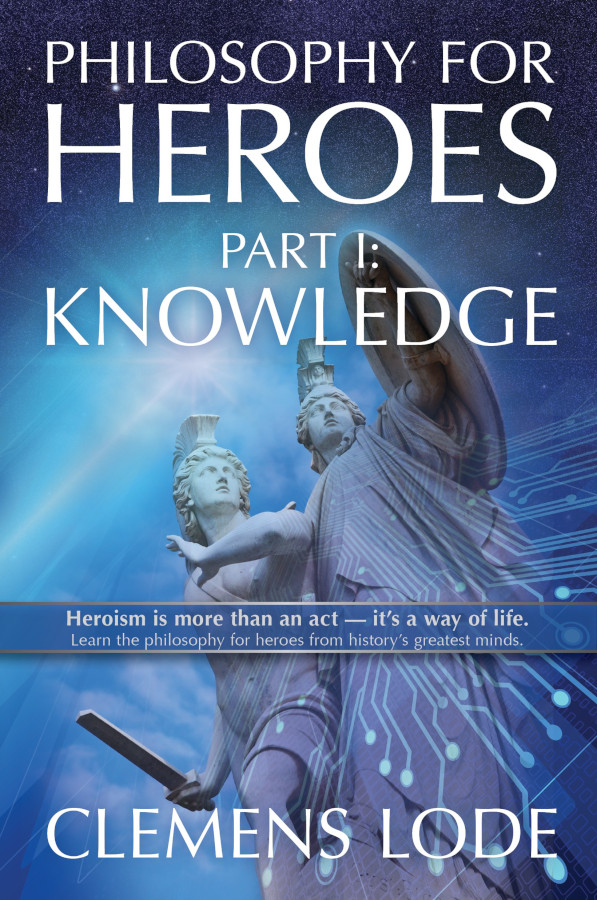
\includegraphics{images/P4H_Cover_12-10-16-front-900.jpg}~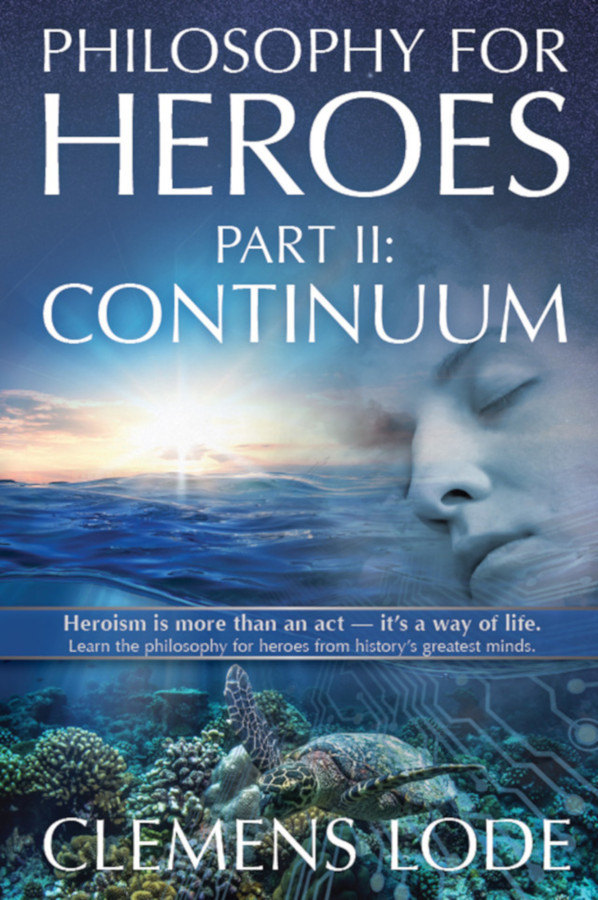
\includegraphics{images/pfh2-cover-900.jpg}
\label{c1_pfh:fig}
\end{figure}

\begin{figure}[H]\centering
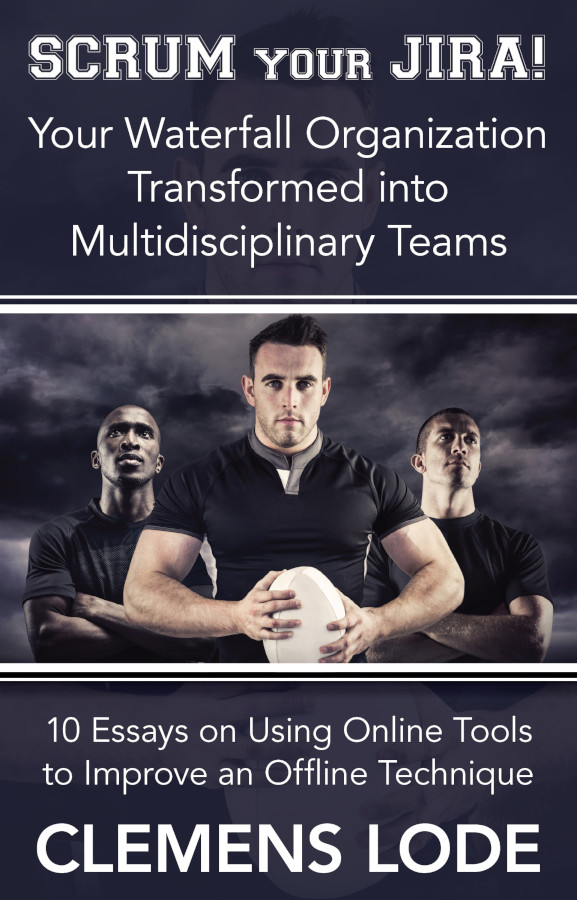
\includegraphics{images/Agile_5-11-17_HiRes2-900.jpg}~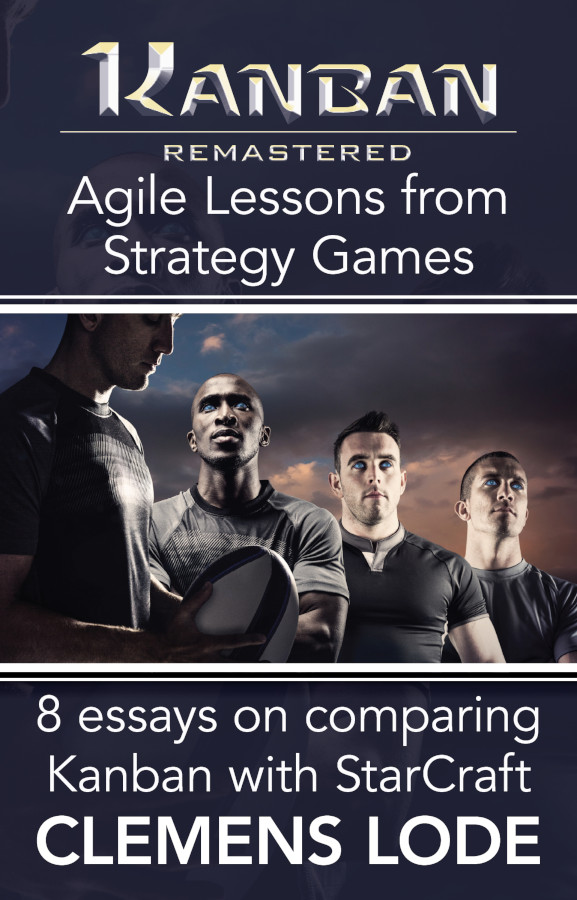
\includegraphics{images/KanbanFront_6-28-17_HiRes-900.jpg}
\label{c1_projectmanagement:fig}
\end{figure}

% Remove the following section if you only want to show your covers, replace with your own book descriptions. The example entries are books I have written using this template.


Here are other books by YOUR NAME. All share the topics of philosophy, psychology, leadership, and project management.

\begin{setlength}{\leftmargin}{1cm} 
\begin{description}\setlength{\itemsep}{-5pt}

\item[Better Books with LaTeX] In \citetitle{BBWL}\index{@\citetitle{BBWL}}\ifxetex\else{} \citep{BBWL}\fi, author Clemens Lode provides you a short-cut into the world of book publishing with \LaTeX{}. It is not a book that just lists all the commands and then leave you alone, it guides you alongside a fully working template (this one!).

\item[Part I: Knowledge.] In \citetitle{PFH1E}\index{@\citetitle{PFH1E}}\ifxetex\else{} \citep{PFH1E}\fi, the first book in this four-book series, author Clemens Lode takes the reader on a journey, examining the foundations of knowledge. What is the basis of our understanding of the world? How does society define a ``hero''? How do basic skills, such as language and mathematics, train our way of thinking and reasoning?

\item[Part II: Continuum.] Beyond the static world of the first book, \citetitle{PFH2E}\index{@\citetitle{PFH2E}}\ifxetex\else{} \citep{PFH2E}\fi{} looks at gradual transitions from one condition to the next. Where do we come from? Why is there something rather than nothing? What is the source of our creativity? How can the study of natural sciences help us to understand who we are?

\item[Scrum Your Jira!] In \citetitle{scrum-your-jira}\index{@\citetitle{scrum-your-jira}}\ifxetex\else{} \citep{scrum-your-jira}\fi, author Clemens Lode challenges two illusions that can get in the way of your company's road to being truly Agile: first, that your Scrum is ``special,'' and second, that you can hide behind project management software. Jira is powerful\emdash{}and this book will show you how to use it more effectively\emdash{}but it makes it easy to forget that the first idea of Agile is: Individuals and interactions over processes and tools.

\item[Kanban Remastered] StarCraft, the most popular real-time strategy game of all time, is also all about producing and deploying just as many game units at just the right time. This book is about the relationship of StarCraft and Kanban. When your team knows StarCraft but not Kanban, \citetitle{kanban-remastered}\index{@\citetitle{kanban-remastered}}\ifxetex\else{} \citep{kanban-remastered}\fi{} will provide you with a series of analogies to allow a better and easier understanding of Agile principles. It is written in a light-hearted tone, similar to how you might chat with a fellow coach about your Agile experiences implementing Kanban, taking for granted that you have experience with StarCraft.

\end{description}
\end{setlength}